\chapter{Evaluation}
\label{chap:evaluation}

This chapter presents performance numbers for Gaia and Syndicate.
Ultimately, the end-to-end performance of an SDS system depends on the decisions
made in the application-specific aggregation and service driver implementations.
 However, each SDS system will impose measurable, predictable overheads on
reads and writes.  It is important for developers to know where these overheads
come from and how big they are in order to make good driver and application design decisions.
In light of the measured overheads, this chapter gives developers
recommendations on how to implement their aggregation drivers to minimize the
impact for specific workloads and end-to-end semantics.

\section{Overview}

SDS systems offer developers a trade-off.  On the one hand, the cost to
developers and users is some additional performance overhead on the read and write paths to cloud services.
This is because the data needs to be converted
into access and mutate flows comprised of manifests and chunks, which must be
relayed through one or more gateways en route to the cloud services.
The SDS metadata service may also need to be contacted in order to
complete the operation.

On the other hand, SDS systems offer significant gains over the status quo.
First, SDS systems greatly reduce the cost of building and maintaining
system-of-systems applications built on cloud services.  By handling storage
semantics and inter-organizational trust relationships
independent of applications, SDS systems allow developers to spend more time on
their application business logic and less time on addressing the users'
storage and trust concerns.  Second, SDS applications
give organizations unilateral control over how
their data is hosted, which frees developers from having to be
responsible for conforming to their hosting policies.
Third, SDS decouples application data from the application
code, preventing users from being locked into relying on a specific
application.  These gains are realized in each
sample application presented in Chapter~\ref{chap:applications}.

Despite overheads, using a SDS system does \emph{not} mean that application workloads take more time or
space than they would had the application avoided SDS.  In fact,
the workload on the SDS system can be \emph{faster} and \emph{require less
space}, depending on the behavior of the service and aggregation drivers.
For example, a service driver can cache blocks on behalf of a slow service like Amazon Glacier~\cite{amazon-glacier},
allowing a read-heavy workload to execute faster with the SDS system
than it would have if the workload had to contact the service directly.
As another example, an aggregation driver can de-duplicate
and compress chunks before sending them to service drivers, speeding up data
transmission and reducing the amount of storage space needed when compared to
directly writing to storage services.

This chapter describes and measures the time and space overheads in both
Syndicate and Gaia's \emph{default} access and mutate flow behaviors, and
provides recommendations on how to design an aggregation driver to minimize
their impact on common workloads.  The measurement focus is on the
\emph{efficiency} of reads and writes---that is, what fraction of time and space
is used for loading and storing the application's data.
Some aggregation driver design recommendations distilled from
these measurements have already been used in real-world applications built
on these SDS systems.

The efficiency measurement gives developers a way to
measure the impact of their service and aggregation driver implementations on
the end-to-end overhead perceived by the application.
A higher efficiency implies higher application-perceived goodput.  Performant
driver implementations maximize efficiency using tactics such as caching
MS-obtained data, or running access and mutate flow steps in parallel when
possible.

To maximize efficiency, the developers need to first understand the SDS system's
overheads in order to make good engineering decisions to minimize their
impact on reads and writes.  But in order to write an effective aggregation
driver, developers need to know what overheads exist in a SDS system first.

\section{Access Flows}

An access flow runs in two steps:  the Discover step translates the
name of a record into a manifest ID, and an Acquire step uses the manifest
ID to fetch the block(s) that contain the requested data.  Both steps may be
implemented in the aggregation driver, but the SDS system supplies a default
implementation if the aggregation driver does not.
This section presents the time and space overheads of the systems' default
access flow behavior, so developers can better understand how to design
aggregation drivers and applications to minimize their effect on their
workflows.

\subsection{Overheads in Gaia}

In both Gaia and Syndicate, the default behavior of the Discover step is to query the
metadata service.  This adds measurable time overhead to the access flow's
execution, comprised of a network round-trip plus the time required by the MS
implementation to look up the current manifest ID for the record.

Gaia is designed for applications where each user is the owner of a volume that
contains all of their application-specific data.
When using a Gaia-powered application, the volume owner usually
has only one device online---the one she is
currently using.  To take advantage of this, Gaia provisions gateways to run 
both the Discover and Acquire step on the volume owner's personal device by
default.  The node itself participates in the peer-to-peer metadata service,
and in doing so maintains a local copy
of all of the users' volume certificate graphs and pointers to Gaia metadata.
In addition, the node maintains a set of service drivers that its gateways can use to load and store
chunks on behalf of the organization that runs it.

The default Discover step in Gaia is to try to fetch the volume record from each
storage system it has a driver for.  This includes
looking up the volume owner's public key and 
certificate graph in the node's local replica of
the system's set of zone files, since this information is required to
authenticate the record.  The volume record itself is stored in the volume
owner's chosen cloud storage services, meaning that the gateway running the
Discover step only has to ask its
node's co-located storage driver to fetch it and decode it.  In the worst case,
the Discover step has to try each storage service before succeeding.

The volume record contains the volume's manifest ID (recall that a Gaia volume
only has a single manifest).  This is passed to the Acquire step, which by
default will fetch each of the volume owner's key space shards in parallel and
reassemble them into the list of keys available in the volume.  Once the full
set of keys are assembled, the Acquire step can finally fetch the requested
value (as a single chunk).

To fetch the value's chunk, the default Acquire step looks at the volume record
to get a list of upstream Gaia gateways or storage providers that the volume
owner has listed as possibly storing a copy.  The Acquire step iterates through
them in order, using one of the node's service drivers to contact each service.
Functionally speaking, the act of asking an upstream Gaia gateway for the chunk is 
equivalent to asking a storage provider---to the requesting
gateway, there is no difference in mechanism (i.e. the upstream gateway is
treated like a storage provider).

To summarize, the sources of overhead in Gaia's default access flows stages are:

\begin{itemize}
\item \textbf{Fetching the volume record in the Discover step}.  This adds both time overhead in
the form of a round-trip to a storage service, and a constant-space overhead from having
to store the volume record (which contains the manifest IDs).
\item \textbf{Fetching the manifest in the Acquire step}.  This
is the work required to find the globally-consistent view of the manifest.
Each device that can write to a Gaia volume stores its own manifest, so a reader
will need to fetch all of them and merge them.  This adds both a time
overhead in the form of a round-trip to a storage service (one per device
manifest), and a $O(kn)$ space overhead for $n$ keys and $k$ devices.  The time overhead of
interest is the combined time
required to fetch all device manifests in parallel, and the time required to authenticate
each device's signature.  The space
overhead is dominated by $n$, since $k$ is the number of devices the volume
owner can use to write (which in practice is small---on the order of 10 or fewer).
Each key requires a constant amount of space.
\item \textbf{Decoding and authenticating the chunk fetched from the Acquire
step}. This adds a time overhead that is $O(n)$ in the number of bytes, since the chunk must
be hashed.
\end{itemize}

\subsubsection{Measured Overheads}

Gaia's read performance was evaluated for records whose sizes vary between 64K
and 640K, in intervals of 64K.  These sizes
were chosen to emulate the sizes of files being stored.  For example, a typical
image would be around 640k (taken from Blockstagram~\cite{blockstagram}),
a typical text document would be around 320k (taken from Graphite
Docs~\cite{graphite-docs}), and the set of the user's
microblog posts would be around 64k (taken from Publik~\cite{publik}).

The read tests were done on a Gaia deployment that matches the \emph{cold start}
default deployment given to each user.
In this deployment, the user runs a local Gaia node that Discovers and Acquires data
from an upstream Gaia node.  The upstream Gaia node loads and stores data from
Microsoft Azure Blob Storage~\cite{azure-blob-storage} in response to downstream
Gaia requests.  Anyone can read from it, but it only accepts writes from users
who have stored profiles that point to at least two social media accounts (i.e.
in order to prevent bots from abusing the system).  In this test, no caching of
any kind was performed by the local Gaia node.

This test evaluates a production deployment of Gaia that serves over
15,000 users.  It is used by the majority of users of the Gaia-powered
applications described in Chapter~\ref{chap:applications}.

An instrumented version of a Gaia node was used to evaluate 150 reads on these
file sizes on the live Gaia network.  A single record was written to an empty
volume and read back 150 times from a single device.
The overall read performance is shown in
Figure~\ref{fig:gaia-read-total}.

\begin{figure}[htp!]
   \centering
   \includegraphics[width=\textwidth]{figures/results/gaia-reads.all/Total}
   \caption{Box-and-whiskers plot of the overall read performance.}
   \label{fig:gaia-read-total}
\end{figure}

Unsurprisingly, the time taken to store data increases linearly with the amount
of data being stored.  Storing a ``small'' file of 64K took a median of 0.836
seconds on the cold path, and an average of 1.56 seconds with a standard
deviation of 1.79.

Each read operation is composed of a Discover and Acquire stage.  The
performance of both of these stages is shown in
Figure~\ref{fig:gaia-read-stages}.

\begin{figure}[htp!]
   \centering
   \begin{subfigure}[b]{.8\textwidth}
      \includegraphics[width=\textwidth]{figures/results/gaia-reads.all/Discover}
      \label{fig:gaia-read-discover}
      \caption{Gaia Discover performance.}
   \end{subfigure}
   \begin{subfigure}[b]{.8\textwidth}
      \includegraphics[width=\textwidth]{figures/results/gaia-reads.all/Acquire}
      \label{fig:gaia-read-acquire}
      \caption{Gaia Acquire performance.}
   \end{subfigure}
   \caption{Box-and-whiskers plots of access flow stage performances in Gaia,
   for file sizes between 64K and 640K in increments of 64K.}
   \label{fig:gaia-read-stages}
\end{figure}

As expected, the Discover stage time overhead is constant relative to the file
size---all that is happening in this stage is the constant-sized 
volume record is being loaded.
Also, as expected, the Acquire stage time increases with file size, since
it includes the times taken to fetch the (single) manifest and fetch the (single) block.
The Acquire stage time overheads are further broken down in
Figure~\ref{fig:gaia-acquire-breakdown}.

\begin{figure}[htp!]
   \centering
   \begin{subfigure}[b]{.8\textwidth}
      \includegraphics[width=\textwidth]{figures/results/gaia-reads.all/GetManifest}
      \label{fig:gaia-read-getmanifest}
      \caption{Times taken to fetch the manifest in the Acquire step, for given
      key/value block sizes.}
   \end{subfigure}
   \begin{subfigure}[b]{.8\textwidth}
      \includegraphics[width=\textwidth]{figures/results/gaia-reads.all/GetBlocks}
      \label{fig:gaia-read-discover}
      \caption{Times taken to fetch the key/value block in the Acquire step, for
      given sizes.}
   \end{subfigure}
   \caption{Box-and-whiskers plots of the Acquire stage performance.}
   \label{fig:gaia-acquire-breakdown}.
\end{figure}

In this test, the manifest size was constant, and took between 0.522 and 0.576 
seconds to download in the median case.  The times taken to download the record
increased with the record size, taking between 0.223 seconds (for 64K) and 0.448
seconds (for 640K) in the median cases.

The efficiency for each read was calculated for record sizes tested.  Two
efficiency results were calculated.  The ``cold efficiency'' is calculated as
the time taken to fetch the record data
divided by the total running time of the access flow.  This includes fetching
the volume record from the underlying cloud storage provider, despite the fact
that in practice this record can be safely cached.  The ``warm efficiency'' is
similar to the ``cold efficiency'', except the total running time of the access
flow \emph{excludes} the time taken to fetch the volume record.  This
calculation reflects the act of caching the volume record.

\begin{figure}[htp!]
   \centering
   \begin{subfigure}[b]{.8\textwidth}
      \includegraphics[width=\textwidth]{figures/results/gaia-reads.all/Efficiency}
      \label{fig:gaia-read-getmanifest}
      \caption{The cold efficiency, which includes the time taken to fetch the
      volume record over the network.}
   \end{subfigure}
   \begin{subfigure}[b]{.8\textwidth}
      \includegraphics[width=\textwidth]{figures/results/gaia-reads.all/Efficiency_cache}
      \label{fig:gaia-read-discover}
      \caption{The warm efficiency, which assumes the volume record is cached
      and excludes it from the access flow's running time}
   \end{subfigure}
   \caption{Box-and-whiskers plots of Gaia's read efficiencies.}
   \label{fig:gaia-read-efficiencies}.
\end{figure}

Both efficiencies are shown in Figure~\ref{fig:gaia-read-efficiencies}.  Naturally,
the efficiencies will tend towards 1.0 for larger and larger record sizes.
However, the act of caching the volume record can significantly improve the read
efficiency for small records.

\subsubsection{Recommendations for Developers}

Relative to fetching data directly from a storage provider, Gaia's most
noticeable time overheads come from fetching and decoding all of the metadata
and volume record information required to request the data.
Fortunately, these costs can be
mitigated by metadata-reading and metadata-writing strategies in
their applications' aggregation drivers.

\hfill \break
\noindent{\textbf{Metadata Caching}}
\hfill \break

In applications that assume at most one writer per login session,
the Gaia gateways can cache data for the duration of the session.
For example, the Gaia-powered Coins application~\cite{coins} assumes that the
user only accesses the data from the same trusted device.  This application's
aggregation driver can
spare users the cost of reloading metadata on each read by having its Acquire
and Publish steps maintain a coherent local copy.

Some applications only need delta-consistency~\cite{delta-consistency}.  In such
applications, users are already expected to have to wait a few seconds for newly-written data to
appear.  In this case, the Acquire step can be implemented to cache metadata for
a particular key for an application-configurable amount of time.  For example, a
social media application could cache the metadata for a user's avatar for a long
time, since it is not expected that the user will change it frequently.  This
would save other readers the cost of having to fetch the same metadata for it 
over and over.

The exact rules for how long to cache a given key/value pair's metadata are
application-specific, and affect the end-to-end storage semantics of the volume.
As such, metadata caching is not part of Gaia's default
behavior.  Instead, Gaia defers to the aggregation driver to make these
decisions.

In practice, the volume record is cached for the duration of the session.  This
was omitted from the read test since the test was meant to
measure overheads from cold starts (in order to identify overhead points).
Simply caching this record for the duration
of a login removes about 0.16 seconds from the read time.

\hfill \break
\noindent{\textbf{Metadata Streaming}}
\hfill \break

Some applications like online shared document editors need to access metadata quickly
from a small set of peers.  In these cases, the Acquire and Publish steps of the
aggregation driver can augment the default read path by eagerly replicating
their metadata via a shared broadcast channel (such as a shared Web socket), in
addition to replicating it to cloud storage.
This way, the Acquire step would listen for Publish events from other peers, and
eagerly update cached metadata before an application read occurs.  If the
broadcast channel is down or starts dropping messages, the Acquire step would fall back
to fetching metadata via the slow path.

Discovering the broadcast channel can be achieved by placing hints in the
volume record in the Gaia MS, such as a set of Websocket URLs.  On loading, the
application would allow the user to connect to other peers by querying the
peers' volume records to find their broadcast channels of choice.

Not all applications need this feature, and even for applications that do need
it, the developer would need to select a broadcast channel that is capable of
handling the application's workload.  As such, Gaia defers
metadata streaming to the aggregation driver implementation.

At least two Gaia-powered applications---Stealthy~\cite{stealthy.im} and
Hermes~\cite{hi-hermes}---are known to use this technique.  Both are
encrypted chat applications, and use a streaming mechanism to accelerate message delivery instead of
forcing clients to continuously poll each others' Gaia volumes.  They
both replicate message logs to Gaia so recipients can read messages
sent to them while they were away.

\subsection{Overheads in Syndicate}

In Syndicate, the Discover and Acquire steps always run on user gateways.
In the default case, the same user gateway runs both
an access flow's Discover and Acquire steps.

The default behavior of Syndicate's Discover step is to contact the
cloud-hosted MS for the latest manifest ID.  Unlike Gaia, Syndicate's
metadata records are arranged into a filesystem-like file hierarchy, and
gateways do not need to obtain a full record of the volume metadata in order to access
blocks.

The time overhead of fetching a given metadata record in Syndicate 
is dependent in how deep into the metadata
hierarchy it is, since at a minimum the user gateway will need to verify that
its cached copies of the path's directory logs are up-to-date.
If the directory's log is not cached or has been modified
since the last request, then the overhead will also include fetching and
synchronizing each directory log in the path.
The space overhead for processing the metadata path 
is simply the sum of the metadata record fetched, plus the
sum of the sizes of the directory logs.

The default behavior of the Acquire step in Syndicate is to first fetch the
manifest from an upstream gateway, and then fetch the relevant blocks from one
or more upstream gateways.  It uses the metadata record from the Discover step
to determine whether or not it needs to contact an acquisition gateway or the
volume's replica gateways.

When reading a record whose data is hosted in a curated dataset, the user
gateway's default Acquire step always contacts the acquisition gateway that
acts as its coordinator.  It determines which gateway this is using the metadata
record acquired in the Discover step.  The acquisition gateway is not given any
any specialized aggregation driver logic by default.  It responds to the user
gateway by using its service
driver to fetch and serve the requested block or manifest from the underlying
data set.

When reading a record whose data is stored in a cloud storage provider, the user
gateway may choose from a set of replica gateways that may be able to access it.
The default behavior of the Acquire step in this case is to ask each replica
gateway in order of increasing gateway ID.  Once the user gateway successfully
fetches the manifest, it fetches at most six blocks in parallel from the replica
gateways.  Similar to how it fetches the manifest, the user gateway will try
contacting each replica gateway in sequence by replica ID for the block (but
will process at most six blocks concurrently).
The choice of six parallel connections is inspired by the same implementation choice made in Web
browsers~\cite{browserscope-browsertest}.  % http://www.browserscope.org/?category=network
The replica gateways are not given any aggregation driver logic for the Acquire
step by default; they simply use their service drivers to fetch and serve chunks
from their services upon request.

To summarize, the overheads in Syndicate's default access flow stages are:

\begin{itemize}
\item \textbf{Synchronizing the metadata path's directory logs}.
In the best case, all of the path entries will be cached and up-to-date.  In
this case, the time overhead is $O(n)$ for $n$ path entries, and $O(dn)$ space
overhead for $d$ entries per directory log.  In the worst case,
all path entries will not be cached.  In this case, both the time and space
overheads are $O(dn)$.
\item \textbf{Fetching blocks and manifests through a replica or acquisition gateway}.  When
servicing an application read, the user gateway does not fetch the data directly
from the cloud service or dataset, but instead contacts an upstream replica
gateway or acquisition gateway to
fetch it on its behalf.  However, this overhead is only
incurred when the user gateway cannot load the requested block or manifest from
an upstream CDN.
\item \textbf{Fetching, authenticating, and decoding the manifest}.
This adds $O(m)$ time and space overhead in the best case (i.e. the first
replica gateway contact has the manifest),
where $m$ is the number of blocks in the record.  In the worst case, the time overhead is
$O(m+r)$ for $r$ replica gateways, since in the worst case the last replica
gateway to be contacted out of the set of replica gateways in the volume
has the manifest.
\item \textbf{Searching for the correct replica gateway}.  Fetching a manifest
or block that is available only from replica gateways incurs at worst a $O(g)$
overhead, for $g$ replica gateways.  This is due to the simple but inefficient
strategy of contacting replica gateways in order by gateway ID.  The $g$
parameter is not expected to change very often relative to the occurrence of reads and
writes, since the user is not expected to frequently add and remove gateways.
\item \textbf{Fetching and decoding the data as a set of blocks}.  A record that exceeds the
volume block size will be fetched piecemeal over HTTP.  This adds $O(n/b)$ time
and space overhead, where $n$ is the number of bytes and $b$ is the block size.
The overheads come from processing and discarding the HTTP headers.  In
addition, each block will be hashed in order to authenticate it,
yielding a $O(n/b)$ time overhead.
\end{itemize}

\subsubsection{Measured Overheads}

Syndicate reads and writes data as fixed-sized blocks.  Obviously, a larger
block size and a larger file size would improve the efficiency of Syndicate
reads and writes, since a greater fraction of the total operation time would be
spent uploading or downloading data.  Therefore, read performance was measured
on a small block size of only 1k, and on a moderate block size of 10k, in order
to emphasize read overheads in the measurements.

File sizes were chosen between 10x and 100x the block size, in intervals of 10
blocks (meaning 10 different file sizes were tested per block size).  Each file
of each size was downloaded 100 times to measure overheads.
The read test was carried out on a volume with one UG and one RG.
The RG and MS ran on a Microsoft
Azure VM and stored metadata and chunks to the VM's local disk.

The Discover step in these tests synchronized one directory (the root) and fetched
one metadata record.  The Acquire step in these tests fetched a manifest representing between 10 and
100 blocks.  The size of the block's metadata in the manifest is
constant---manifest sizes and download times are a function of the number of
blocks only.  However, the size of the record metadata on the MS increases with
the number of blocks, since the MS stores a garbage-collection log for all
blocks in the record.  Each garbage-collection entry is only 8 bytes.


\begin{figure}[htp!]
   \centering
   \begin{subfigure}[b]{.8\textwidth}
      \includegraphics[width=\textwidth]{figures/results/syndicate-writes.1024.all/Total}
      \label{fig:syndicate-read-total-1k}
      \caption{Syndicate access flow performance with 1K blocks}
   \end{subfigure}
   \begin{subfigure}[b]{.8\textwidth}
      \includegraphics[width=\textwidth]{figures/results/syndicate-writes.10240.all/Total}
      \label{fig:syndicate-read-total-1k}
      \caption{Syndicate access flow performance with 10K blocks}
   \end{subfigure}
   \caption{Box-and-whiskers plots of end-to-end access flow performances in
   Syndicate, for 1K and 10K block sizes.}
   \label{fig:syndicate-read-total}
\end{figure}

The total read performances for 1K and 10K block sizes are shown in
Figure~\ref{fig:syndicate-read-total}.  These represent the times taken by all
of the Discover and Acquire logic, including the aforementioned overheads.

\begin{figure}[htp!]
   \centering
   \begin{subfigure}[b]{.8\textwidth}
      \includegraphics[width=\textwidth]{figures/results/syndicate-reads.1024.all/Discover}
      \label{fig:syndicate-read-discover-1k}
      \caption{Syndicate Discover performance with 1K blocks}
   \end{subfigure}
   \begin{subfigure}[b]{.8\textwidth}
      \includegraphics[width=\textwidth]{figures/results/syndicate-reads.1024.all/Acquire}
      \label{fig:syndicate-read-acquire-1k}
      \caption{Syndicate Acquire performance with 1K blocks}
   \end{subfigure}
   \caption{Box-and-whiskers plots of access flow stage performances in
   Syndicate, for file sizes between 10K and 100K and a block size of 1K.}
   \label{fig:syndicate-read-stages-1K}
\end{figure}

\begin{figure}[htp!]
   \centering
   \begin{subfigure}[b]{.8\textwidth}
      \includegraphics[width=\textwidth]{figures/results/syndicate-reads.10240.all/Discover}
      \label{fig:syndicate-read-discover-10k}
      \caption{Syndicate Discover performance with 10K blocks}
   \end{subfigure}
   \begin{subfigure}[b]{.8\textwidth}
      \includegraphics[width=\textwidth]{figures/results/syndicate-reads.10240.all/Acquire}
      \label{fig:syndicate-read-acquire-1k}
      \caption{Syndicate Acquire performance with 10K blocks}
   \end{subfigure}
   \caption{Box-and-whiskers plots of access flow stage performances in
   Syndicate, for file sizes between 100K and 1000K and a block size of 10K.}
   \label{fig:syndicate-read-stages-10K}
\end{figure}


Figures~\ref{fig:syndicate-read-stages-1K} and \ref{fig:syndicate-read-stages-10K}
show the Discover and Acquire stage performances of Syndicate access flows for 1K and
10K blocks, respectively.
In both cases, the times taken by the Discover step increase slightly for
records with 80, 90, and 100 blocks.  This is due to the fact that the MS
incurs extra disk overhead from loading the a metadata record with a larger
garbage-collection log.  This could be optimized away.

Unsurprisingly, the Acquire stages increase in time as a linear function of the
number of blocks fetched.  The spreads of the distributions increase
with the number of blocks because more blocks introduce more noise into the
measurement.  The time taken to fetch records increases faster for 10K blocks
than for 1K blocks.


\begin{figure}[htp!]
   \centering
   \begin{subfigure}[b]{.8\textwidth}
      \includegraphics[width=\textwidth]{figures/results/syndicate-reads.1024.all/GetManifest}
      \label{fig:syndicate-getmanifest-1k}
      \caption{Syndicate's performance of fetching manifests with 1K blocks}
   \end{subfigure}
   \begin{subfigure}[b]{.8\textwidth}
      \includegraphics[width=\textwidth]{figures/results/syndicate-reads.1024.all/GetBlocks}
      \label{fig:syndicate-getblocks-1k}
      \caption{Syndicate's performance of fetching records of various sizes with
      1K blocks.}
   \end{subfigure}
   \caption{Box-and-whiskers plots of Syndicate's Acquire stage performance with 1K
   blocks.}
   \label{fig:syndicate-acquire-breakdown-1K}
\end{figure}

\begin{figure}[htp!]
   \centering
   \begin{subfigure}[b]{.8\textwidth}
      \includegraphics[width=\textwidth]{figures/results/syndicate-reads.10240.all/GetManifest}
      \label{fig:syndicate-getmanifest-10k}
      \caption{Syndicate's performance of fetching manifests with 10K blocks}
   \end{subfigure}
   \begin{subfigure}[b]{.8\textwidth}
      \includegraphics[width=\textwidth]{figures/results/syndicate-reads.10240.all/GetBlocks}
      \label{fig:syndicate-read-acquire-1k}
      \caption{Syndicate's performance of fetching the blocks for records of various sizes with
      10K blocks.}
   \end{subfigure}
   \caption{Box-and-whiskers plots of Syndicate's Acquire stage performance with
   10K blocks.}
   \label{fig:syndicate-acquire-breakdown-10K}
\end{figure}

The tasks of fetching the manifest ID and fetching
the blocks for the Acquire stages are further broken down in
Figures~\ref{fig:syndicate-acquire-breakdown-1K} and
\ref{fig:syndicate-acquire-breakdown-10K}.

The times taken to fetch the manifests are about the same across the record
and block sizes sizes measured.  While
the size of a manifest grows linearly with the number of blocks, it does so via
a small constant factor per block (48 bytes per block).  The times taken to
fetch the blocks are the reason why the Acquire stage's time increases linearly
with the record size.

\begin{figure}[htp!]
   \centering
   \begin{subfigure}[b]{.8\textwidth}
      \includegraphics[width=\textwidth]{figures/results/syndicate-reads.1024.all/Efficiency}
      \label{fig:syndicate-cold-efficiency-1k}
      \caption{The cold efficiency for 1K blocks, which includes the time taken to fetch the
      metadata record from the MS.}
   \end{subfigure}
   \begin{subfigure}[b]{.8\textwidth}
      \includegraphics[width=\textwidth]{figures/results/syndicate-reads.1024.all/Efficiency_cache}
      \label{fig:syndicate-warm-efficiency-1k}
      \caption{The warm efficiency, which assumes the metadata record is cached
      and excludes it from the access flow's running time}
   \end{subfigure}
   \caption{Box-and-whiskers plots of Syndicate's read efficiencies for 1K blocks.}
   \label{fig:syndicate-read-efficiencies-1k}
\end{figure}

\begin{figure}[htp!]
   \centering
   \begin{subfigure}[b]{.8\textwidth}
      \includegraphics[width=\textwidth]{figures/results/syndicate-reads.10240.all/Efficiency}
      \label{fig:syndicate-cold-efficiency-10k}
      \caption{The cold efficiency for 1K blocks, which includes the time taken to fetch the
      metadata record from the MS.}
   \end{subfigure}
   \begin{subfigure}[b]{.8\textwidth}
      \includegraphics[width=\textwidth]{figures/results/syndicate-reads.10240.all/Efficiency_cache}
      \label{fig:syndicate-warm-efficiency-10k}
      \caption{The warm efficiency, which assumes the metadata record is cached
      and excludes it from the access flow's running time}
   \end{subfigure}
   \caption{Box-and-whiskers plots of Syndicate's read efficiencies for 10K blocks.}
   \label{fig:syndicate-read-efficiencies-10k}
\end{figure}

Figures~\ref{fig:syndicate-read-efficiencies-1k} and
\ref{fig:syndicate-read-efficiencies-10k} plot the cold and warm efficiencies of
Syndicate, for 1K blocks and 10K blocks respectively.  In both cases, the
efficiencies approach 1.0 as the record sizes increases.  The warm efficiency
excludes the time taken to fetch the metadata record from the MS (i.e. by
caching it locally).  Caching metadata makes a noticeable difference in the
system's efficiency for small files---it can be up to 33% higher.

\subsubsection{Recommendations for Developers}

Syndicate gives developers several options to manage read performance in the
face of these overheads.  A few of these recommendations have been put into
practice in production settings.

\hfill \break
\noindent{\textbf{Long Metadata TTL with Explicit Invalidation}}
\hfill \break

Volumes of scientific data often have few writers.  In cases where a volume is
backed by a dataset, the only writer would be the acquisition gateway that
crawls the dataset.  In cases where a volume acts as a data dump or a scratch space,
writes happen only when a workload finishes, and occur on the same set of
metadata paths (e.g. each user or each workflow would write its dump to its own
directory).

Developers can take advantage of these special cases to save round-trips to the MS.
The Publish steps of writer gateways can be programmed to 
broadcast a metadata invalidation hint to all read-capable gateways in the
volume.  The MS would only be contacted as a fallback.

This strategy is used in the scientific data-sharing application today in order
to improve the efficiency of reading small files.

\hfill \break
\noindent{\textbf{Use a CDN}}
\hfill \break

Syndicate was designed to be used with a CDN.  Developers wishing to get the
best read performance would implement their Acquire step to contact one or more
CDNs that can pull down chunks from upstream replica gateways.  This is highly
beneficial for read-heavy workloads, where most of the chunks can be cached
close to readers.  This reduces the number of network round-trips and reduces
the amount of transit traffic out of cloud storage providers, all without
violating end-to-end storage semantics and organizational autonomy.

The performance boost developers can expect to see depends on the CDN leveraged
and the size of the working set.
However, the benefit to breaking data into chunks is that
developers can expect the CDN to accelerate reads even if only
part of the data is cached.

This strategy is used in the scientific data-sharing application today.  The
CDN---an instance of the Akamai~\cite{akamai} CDN---is deployed on OpenCloud~\cite{opencloud}.

\hfill \break
\noindent{\textbf{Gateway-local Block Cache}}
\hfill \break

Since Syndicate handles end-to-end semantics at a level above block transport,
each gateway can implement a write-coherent block cache in its Acquire stage. 
This effectively adds multiple tiers to a commodity CDN---the first tier would be at the user
gateways, the CDN would be the shared middle tier, and the replica and acquisition
gateways would be the top tier.  Syndicate gateways offer this feature as a
built-in option, but using it requires the developer to set the cache size first
(which is workload-specific).

This strategy is deployed in the scientific data-sharing application.

\hfill \break
\noindent{\textbf{Chunk Advertisement}}
\hfill \break

If the developer implements a gateway-local block cache in the Acquire step, a
complementary feature would be allowing gateways to advertise to one another
which chunks they have cached.  If the Acquire step detects that a nearby peer
has a cached chunk, then it could fetch the chunk from the nearby peer instead
of from an upstream cache.  This is useful in cluster computing, where
host-to-host bandwidth is high but bandwidth in and out of the cluster is
comparatively low.  It may be cheaper to fetch a chunk from a cluster peer than
an upstream CDN node.

This strategy is also useful for MapReduce~\cite{mapreduce}-style
workflows, where the job scheduler can query gateways to determine
which chunks are already cached so it can schedule jobs on hosts that already
have the requisite data.  This is a feature implemented in Syndicate's HDFS driver, for
example.

This is not part of the default behavior because it makes assumptions about the
network bandwidth between gateways and assumptions about the threat model the
deployment faces.  A wide-area Syndicate volume would not want this feature,
because it would disclose to the Internet information about which gateways could
access which data, and thus give an attacker insight into which hosts
to compromise in order to exfiltrate it.

\hfill \break
\noindent{\textbf{Chunk Compression}}
\hfill \break

Syndicate gives developers the ability to control the wire-format of each chunk.
If the entropy of the data is low, then developers stand to gain by having their
gateways' \texttt{serialize()} and \texttt{deserialize()} driver methods
compress and decompress chunks.  However, if the data has high entropy, then
this strategy would be useless.  Syndicate does not do this by default, but
instead defers to developers to make the right decision based on their data.

\hfill \break
\noindent{\textbf{Read-ahead}}
\hfill \break

Many scientific workflows read sequentially.  If this is the application's
behavior, then the developer can program the Acquire step to pre-fetch blocks
asynchronously.  This is useful if the application is reading
variable-sized ranges of a file that straddle block boundaries---the last block
fetched in one read will be the first block fetched in the next read, so keeping
it local would save a round-trip.

Syndicate does not perform read-ahead by
default because it cannot assume that data reads are sequential.  In a
random-read workload, read-ahead would be more wasteful than the default
behavior.  However, if  the developers know that their application has a
read-sequential access pattern, then they can add this behavior to the Acquire
stage.

\hfill \break
\hfill \break
\noindent{\textbf{Favor Shallow Metadata Hierarchies}}
\hfill \break

Developers can reduce the amount of time spent querying metadata by organizing
their data into shallow directory hierarchies.  This would cut down on the
number of round-trips to the MS to resolve a path.  In addition, developers can
ensure that their directories do not get too big in order to minimize the
cold-cache start-up time for a user gateway to synchronize its metadata logs.

This strategy is used in the scientific data-sharing application.

\section{Mutate Flows}

A mutate flow has three steps:  a Build step which constructs a new manifest
for a record that incorporates the modified blocks, a Push step which replicates
the new manifest and new blocks, and a Publish step which makes the mutation
visible to subsequent access flows.  A SDS system supplies default
implementations of these steps, but they may be overwritten by the aggregation
driver.  This section presents the time and space overheads the default steps in
Gaia and Syndicate impose on top of application writes, and presents a
discussion on how developers can minimize them.

\subsection{Overheads in Gaia}

To handle writes, Gaia's default strategy to process a
mutate flow is to do so entirely on the volume owner's device.  When the volume
owner signs into the application, the device's Gaia node instantiates gateways with the Build,
Push, and Publish stages in order to service application writes for this session.

The Build stage takes the new key/value pair the application is trying to write,
and assembles a new key space shard to replicate.  The Push stage takes the
key's value and replicates it to the volume's cloud storage
services.  This may include Pushing them to an upstream Gaia node, which carries
out further processing (but to the node doing the Push, the upstream Gaia node
looks and behaves like another cloud storage service).  The Publish stage takes
the new key space shard and replicates it alongside the Pushed key value.

The default deployment of Gaia implements a couple of optimizations.
First, the Gaia node optimizes the execution of a mutate flow as a sequence
of subroutine calls.  There is minimal overhead between passing control from a
Build stage to a Push stage, and from a Push stage to a Publish stage.
Second, the Push and Publish stages execute in parallel by default.  This is
because there often no logical dependencies between them that require them
to run sequentially.

The end-to-end default write overheads include:

\begin{itemize}
\item \textbf{The time and space overheads of generating the new metadata}.  In
the Build step, the Gaia node will need to hash the key/value pair
chunk and append it to the manifest.  This adds a $O(n)$ time overhead, where
$n$ is the size of the value.  In addition, the Gaia node will need to ensure
that it has a fresh copy of the key shard before it can build a new key
shard (i.e. before the mutate flow executes, another mutate flow may have
executed from another one of the user's devices).
\item \textbf{The time and space overheads in storing the new key shard}.  Each new
key added takes $O(1)$ additional space to the volume's manifest, and $O(1)$
additional space to the volume's metadata.
Storing the key shard adds a $O(n)$ time and space overhead for $n$ records in the volume
(since in the worst case, a key shard can have as many records as there are
keys in the volume).  These costs are incurred in the Publish step, where the
volume's manifest is replicated.
\end{itemize}

\subsubsection{Measured Overheads}

Write overheads in Gaia were measured on the live Gaia network.  Just as with
the read experiment, this test was conducted on a representative Gaia deployment
whereby the user runs a local Gaia node that will Push and Publish new data to
an upstream Gaia node, which in turn Pushes the data (as chunks) to a bucket in
Microsoft Azure.

The test wrote key/value pairs with sizes ranging between 64K and 640K, in
intervals of 64K, to simulate writing
data from real-world Gaia applications.  The test wrote the files 150 times
using an instrumented Gaia node to measure overheads.  Each run was from a cold
start---there was no caching performed between requests.

\begin{figure}[htp!]
   \centering
   \includegraphics[width=\textwidth]{figures/results/gaia-writes.all/Total}
   \caption{Box-and-whiskers plot of the overall write performance.}
   \label{fig:gaia-write-total}
\end{figure}

The overall write performance for Gaia is shown in
Figure~\ref{fig:gaia-write-total}.  While the measurement is noisy, the write
times increase linearly with the file size.  The source of the noise comes from
the fact that the upstream Gaia node is shared with many Gaia users.

\begin{figure}[htp!]
   \centering
   \begin{subfigure}[b]{.8\textwidth}
      \includegraphics[width=\textwidth]{figures/results/gaia-writes.all/Build}
      \label{fig:gaia-write-build}
      \caption{Gaia Build performance.  Note that this includes the cost of
      fetching the existing manifest before constructing a new one.}
   \end{subfigure}
   \begin{subfigure}[b]{.8\textwidth}
      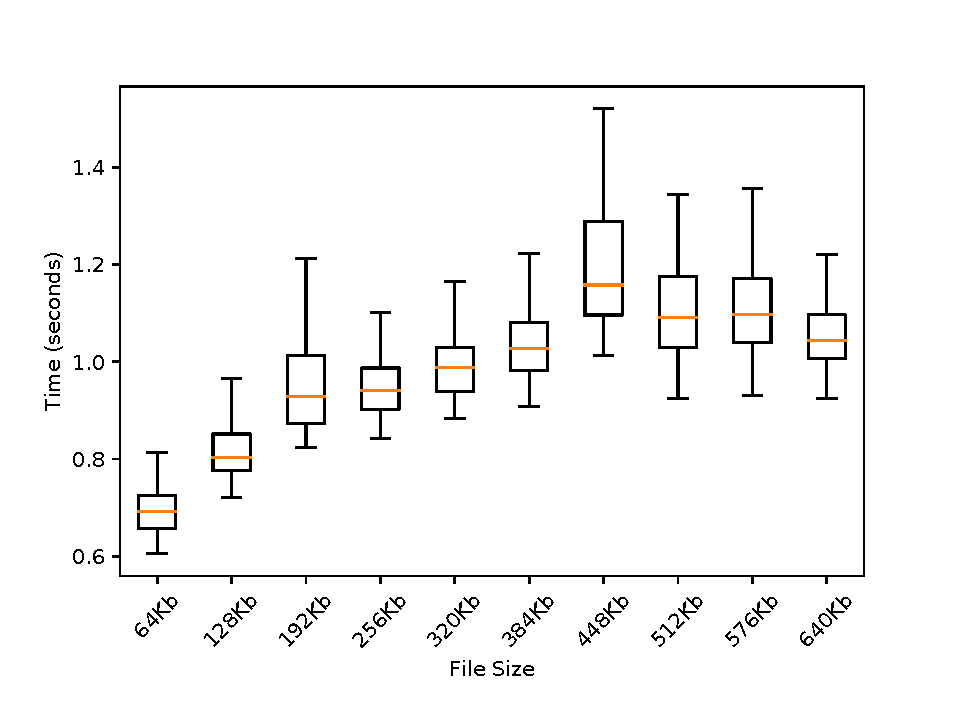
\includegraphics[width=\textwidth]{figures/results/gaia-writes.all/PushPublish}
      \label{fig:gaia-write-pushpublish}
      \caption{Gaia Push/Publish performance (both stages execute in parallel).}
   \end{subfigure}
   \caption{Box-and-whiskers plots of mutate flow stage performances in Gaia,
   for file sizes between 64K and 640K in increments of 64K.}
   \label{fig:gaia-write-stages}
\end{figure}

Figure~\ref{fig:gaia-write-stages} shows the Build, Push, and Publish stage
performances in Gaia.  In this test, the Build stage includes
the time taken to fetch a copy of the device manifest to update.  If the device
manifest is cached, then the Build stage is extremely fast---effectively the amount of
time taken to hash the data and insert it into a hash table and serialize the
hash table to a string for upload.

The Push and Publish stages run in parallel in Gaia by default, so their
measurements are combined.

\begin{figure}[htp!]
   \centering
   \begin{subfigure}[b]{.8\textwidth}
      \includegraphics[width=\textwidth]{figures/results/gaia-writes.all/Efficiency}
      \label{fig:gaia-read-getmanifest}
      \caption{The cold efficiency, which includes the time taken to fetch the
      volume record over the network.}
   \end{subfigure}
   \begin{subfigure}[b]{.8\textwidth}
      \includegraphics[width=\textwidth]{figures/results/gaia-writes.all/Efficiency_cache}
      \label{fig:gaia-read-discover}
      \caption{The warm efficiency, which assumes the volume record is cached
      and excludes it from the mutate flow's running time}
   \end{subfigure}
   \caption{Box-and-whiskers plots of Gaia's write efficiencies.}
   \label{fig:gaia-write-efficiencies}.
\end{figure}

This test calculated the efficiency of Gaia's write path in two ways---a ``cold
write efficiency'' which includes the cost of fetching the manifest in the Build
stage, and a ``warm write efficiency'' which excludes this step.  Including both
efficiency measures is valuable to developers because often times, the manifest
can be safely cached across writes.  Figure~\ref{fig:gaia-write-efficiencies}
reports both cold and warm efficiencies.  The efficiency of the write path
improves somewhat when the manifest can be cached across writes.

\subsubsection{Recommendations to Developers}

Developers have a few strategies available to alter the performance of writes in Gaia.
The specific strategies taken ultimately depend on the workload and data being
stored.

\hfill \break
\noindent{\textbf{Incremental Key Space Shard Writes}}
\hfill \break

Some applications may have a large key space, but only need to carry out a
key/value writes at a time.
The aggregation driver has an opportunity to reduce the amount of time and space that
need to be consumed to carry the write out by only writing the new key metadata.

If the application only wrote one value, then only one key in the manifest would
be altered.  The Build stage could be optimized to inspect the Gaia node's 
key space shard in-between writes, only pass along the delta between writes
to the Push stage.

The Push stage would accumulate deltas from the Build stage, and combine them
into a single key shard in the backend storage service.  Then, a subsequent
Acquire step would continue to fetch the key space shard as expected.

The reason this is not the default behavior is because patching a record
efficiently requires the cloud service to support a ``range write''
API call, whereby the client specifies a byte offset and length as to where to
write the given data.  Most popular cloud storage providers do not support
this---they only allow clients to write whole records.  For these services,
a Push stage could not efficiently write key shard deltas, since it would need
to load the entire key shard, patch it, and store the entire updated key shard
on each write.  As such, this behavior would be added by developers in the
special case where they were using a suitable cloud storage provider.

\hfill \break
\noindent{\textbf{Write Batching}}
\hfill \break

Applications may not need all of their writes to be Published immediately.
Instead, a Publish can reflect many writes at once.  This would be allowed if
the application's storage semantics do not require all peers to see each others'
most-recent state.  This can lead to better overall performance for applications
that frequently overwrite the same key/value pairs---overwritten key/value pairs
would not need to be replicated.

Applications that have semantics compatible with write-batching can not only
realize better performance than the default behavior, but also take advantage of
client-side libraries that offer more expressive storage interfaces.
Examples include Compass~\cite{blockstack-compass}, which provides a
MongoDB-like interface, and \texttt{sql.js}~\cite{sql.js}, which provides a
client-side SQLite implementation.  Both of these libraries are easily used with
Gaia, provided that the application's storage semantics allow write-batching
(i.e. a Publish would take place in response to the application committing a
transaction in one of these APIs).  In fact, Compass was designed specifically
for Gaia by a third party contributor.

\subsection{Overheads in Syndicate}

Syndicate's default write strategy is make data as durable as possible. 
This is realized by the default behaviors of replicating all
manifests and blocks to all replica gateways in the volume in the
Push stage, and synchronously uploading the record's metadata to the Syndicate
MS in the Publish stage.

User gateways invoke the Build, Push, and Publish stages on write.
Since Syndicate is designed to process scientific workloads, it expects
multiple write-capable user gateways to be online at once.  However, it assumes
that user gateways usually (but not always) write to the same files that they
coordinate.  This is reasonable in practice, since scientific computing loads
are usually designed to run on many parallel computers which share as little
data with one another as possible.

In light of this, the default common-case behaviors of the Build, Push, and
Publish stages in Syndicate are to assemble a new manifest locally (Build),
replicate the manifest and blocks to all replica gateways (Push), and
synchronously upload the new metadata to the MS (Publish).  Push and Publish are
run automatically when a record is \texttt{close()}'ed, if the application does
not do so explicitly via a call to \texttt{fsync()}.  These are the default
behaviors of the user gateway carrying out the write is also the coordinator.

If the writer gateway is not the coordinator, then it enlists the
coordinator's help it carry out the write.  The writer's Push stage will first
replicate the new blocks, and then synchronously request that the coordinator
both Push a new manifest with the requested changes
and Publish new metadata that reflects it.

By default, replica gateways do not have any specialized aggregation driver
logic on the write path.
They simply accept chunks from user gateways, and replicate them with
their service drivers.

To summarize, the write overheads in Syndicate are as follows:

\begin{itemize}
\item \textbf{The time and space overheads of building a new manifest}.  By
default, a UG will incur a network round-trip when it Builds a new manifest for a record that
it does not coordinate.  In addition, the UG will incur a round-trip to
the MS to ensure that the new manifest it is modifying is fresh when executing
the default Build implementation.
\item \textbf{The time and space overheads of storing new metadata}.  The
record's coordinator will incur a network round-trip to the MS when Publishing
new data, and storing the new metadata incurs $O(1)$ extra space.  In the case
where the writer is not the coordinator, two network round-trips are incurred:
one to the MS and back, and one to the coordinator and back.
\item \textbf{The time and space overheads of storing a new manifest}.  The
record's coordinator will incur a network round-trip to each replica gateway to
store the new manifest, and a network round-trip from each replica gateway to
its underlying storage services.  This yields $O(g)$ round-trips, where $g$ is the number of
replica gateways.  The manifest size is $O(n)$ bytes for a record of $n$ bytes,
so replicating and storing it to all gateways takes $O(gn)$ time and space.
\item \textbf{The time overheads of storing blocks}.  Similar to manifests,
replicating a block takes two network round-trips (one for the replica gateway,
and one for the service).
\end{itemize}

\subsubsection{Measured Overheads}

The overheads of writing in Syndicate were measured for the same block sizes and
record sizes as reads:  records composed of 10 to 100 blocks (in intervals of 10
blocks) for a ``small'' block size of 1K and a ``medium'' block size of 10K.
The same UG, RG, and MS in the read test were used in the write test.
The total mutate flow performances are shown in
Figure~\ref{fig:syndicate-writes-total}.

\begin{figure}[htp!]
   \centering
   \begin{subfigure}[b]{.8\textwidth}
      \includegraphics[width=\textwidth]{figures/results/syndicate-writes.1024.all/Total}
      \label{fig:syndicate-read-discover-1k}
      \caption{Syndicate mutate flow performance with 1K blocks}
   \end{subfigure}
   \begin{subfigure}[b]{.8\textwidth}
      \includegraphics[width=\textwidth]{figures/results/syndicate-writes.1024.all/Total}
      \label{fig:syndicate-read-acquire-1k}
      \caption{Syndicate mutate flow performance with 10K blocks}
   \end{subfigure}
   \caption{Box-and-whiskers plots of mutate flow performances in
   Syndicate, for file sizes between 10K and 100K and a block size of 1K.}
   \label{fig:syndicate-writes-total}
\end{figure}

Despite the noisy measurements, the amount of time taken to write records of
these sizes grows linearly with file size.  For the 1K block measurement, the noise in the
measurements is mainly due to variations in the disk write performance and
chunk-writing scheduler in the UG.  For the 10K block measurement, the noise is
mainly due to the Push stage (i.e. there is more variance in uploading large
blocks).  This is visible in the Build, Push, and Publish
performances in Figures~\ref{fig:syndicate-build}, \ref{fig:syndicate-push}, and
\ref{fig:syndicate-publish}, respectively.

\begin{figure}[htp!]
   \centering
   \begin{subfigure}[b]{.8\textwidth}
      \includegraphics[width=\textwidth]{figures/results/syndicate-writes.1024.all/Build}
      \label{fig:syndicate-build-1k}
      \caption{Syndicate Build stage performance with 1K blocks}
   \end{subfigure}
   \begin{subfigure}[b]{.8\textwidth}
      \includegraphics[width=\textwidth]{figures/results/syndicate-writes.10240.all/Build}
      \label{fig:syndicate-build-10k}
      \caption{Syndicate Build stage performance with 10K blocks}
   \end{subfigure}
   \caption{Box-and-whiskers plots of the Build stage performance, for 1K and
   10K blocks.}
   \label{fig:syndicate-build}
\end{figure}

The Build step occurs within the UG.  In Syndicate, the Build step includes the
process of hashing the blocks and flushing them to a temporary storage location on
disk before it is replicated.  While the effect is hard to see here due to the 
small amount of data, the Build stage's time increases linearly with the amount
of data being written, since the manifest includes the hashes of all blocks
(Figure~\ref{fig:syndicate-build}).  The Build stage with 1K blocks completes in
less than 500 milliseconds, while the Build stage with 10K blocks takes less
than 750 milliseconds.

\begin{figure}[htp!]
   \centering
   \begin{subfigure}[b]{.8\textwidth}
      \includegraphics[width=\textwidth]{figures/results/syndicate-writes.1024.all/Push}
      \label{fig:syndicate-push-1k}
      \caption{Syndicate Push stage performance with 1K blocks}
   \end{subfigure}
   \begin{subfigure}[b]{.8\textwidth}
      \includegraphics[width=\textwidth]{figures/results/syndicate-writes.10240.all/Push}
      \label{fig:syndicate-push-10k}
      \caption{Syndicate Push stage performance with 10K blocks}
   \end{subfigure}
   \caption{Box-and-whiskers plots of the Push stage performance, for 1K and
   10K blocks.}
   \label{fig:syndicate-push}
\end{figure}

The Push stage replicates all blocks to the RG.  The Push stage times show linear
increases with the number of blocks (Figure~\ref{fig:syndicate-push}).
In the 1K block size case, the median Push stage
completes within 1.9 and 2.5 seconds.  In the 10K block size case, the median
Push stage completes within 3.5 and 8.1 seconds.

\begin{figure}[htp!]
   \centering
   \begin{subfigure}[b]{.8\textwidth}
      \includegraphics[width=\textwidth]{figures/results/syndicate-writes.1024.all/Publish}
      \label{fig:syndicate-publish-1k}
      \caption{Syndicate Publish stage performance with 1K blocks}
   \end{subfigure}
   \begin{subfigure}[b]{.8\textwidth}
      \includegraphics[width=\textwidth]{figures/results/syndicate-writes.10240.all/Publish}
      \label{fig:syndicate-publish-10k}
      \caption{Syndicate Publish stage performance with 10K blocks}
   \end{subfigure}
   \caption{Box-and-whiskers plots of the Publish stage performance, for 1K and
   10K blocks.}
   \label{fig:syndicate-publish}
\end{figure}

The Publish stage replicates the new manifest ID to the MS, as well as a
garbage-collection log.  Because the garbage-collection log data that the UG
replicates is proportional to the number of blocks written, it is expected that
the amount of time taken to replicate metadata will increase linearly with the
size of the write.

However, due to the facts that only at most 100 blocks are replicated and that
the size of a garbage-collection entry is 8 bytes, this linear relationship is
not visible.  Publish steps take between 640 milliseconds and 900 milliseconds
across both the 1K and 10K block size tests
(Figure~\ref{fig:syndicate-publish}).

\begin{figure}[htp!]
   \centering
   \begin{subfigure}[b]{.8\textwidth}
      \includegraphics[width=\textwidth]{figures/results/syndicate-reads.1024.all/Efficiency}
      \label{fig:syndicate-efficiency-1k}
      \caption{Syndicate write efficiency for 1K blocks.}
   \end{subfigure}
   \begin{subfigure}[b]{.8\textwidth}
      \includegraphics[width=\textwidth]{figures/results/syndicate-reads.10240.all/Efficiency}
      \label{fig:syndicate-efficiency-1k}
      \caption{Syndicate write efficiency for 10K blocks.}
   \end{subfigure}
   \caption{Box-and-whiskers plots of the efficiencies of Syndicate
   writes.}
   \label{fig:syndicate-write-efficiency}
\end{figure}

The write efficiencies of Syndicate are shown in
Figure~\ref{fig:syndicate-write-efficiency}.  As long as internal fragmentation
can be avoided, using larger block sizes drastically improves the system's
efficiency.

\subsubsection{Recommendations for Developers}

In addition to recommendations for aggregation driver developers for reads, some
performance enhancements can be devised for writes.  These strategies depend on
the workload and the nature of the data, which is why they are not included in
the default behavior.

\hfill \break
\noindent{\textbf{Write Coalescing}}
\hfill \break

A lot of workflows write data sequentially, and in bursts.
Developers can save a set of round-trips to the replica gateways
in the case where two sequential writes straddle a block boundary
by deferring replication of the straddled block.

\hfill \break
\noindent{\textbf{Replica Gateway Selection}}
\hfill \break

Developers are not required to replicate a chunk to all gateways.  It is
expected that in situations where there are multiple choices for a data store,
the aggregation driver will choose which chunk goes with which storage provider.
This can be done both to preserve end-to-end storage semantics, and to improve
write performance.

\hfill \break
\noindent{\textbf{Replica Gateway Chains}}
\hfill \break

Syndicate supports custom gateway types.  Developers can exploit this
to implement chain replication~\cite{chain-replication}~\cite{craq}, whereby a set of 
replica gateways are arranged into a sequence such that when receiving a chunk,
the gateway stores it and forwards it to the next gateway in the sequence.
User gateways would only need to forward chunks to the chain tip.  The tip would
have a ``replica gateway'' type, but the gateways in the chain would have a
distinct ``chain replicator'' type.

The aggregation driver would be written
such that each replica gateway and chain replicator gateway discover their
types and locations in the topology from the certificate graph.  The Push stage
for each gateway would use this knowledge to determine its next-hop gateway.
This strategy is generalizable to arbitrary store-and-forward topologies.

The performance advantage this would incur is that it would enable the same
degree of durability as replicating in parallel, but without the extra
round-trips from the user gateway.  User gateways located behind
underprovisioned network links would notice the improvement, since they would
not need to spend as much time pushing chunks through a local bottleneck.

\hfill \break
\noindent{\textbf{Chunk Patching}}
\hfill \break

If the workload exhibits random-write behaviors, one strategy developers can
employ is to implement a ``patching'' algorithm in their aggregation driver's
Push stage.  Instead of sending the entire chunk to a replica gateway, a user
gateway would send only the byte ranges and offsets to the replica gateways.
This would cut down on the data the replica gateway needs to send, even if the
block size in the volume was large.
The replica gateway would reassemble the patches into a block sometime before
the next read occurs---either eagerly as part of an internal
garbage-collection algorithm, or lazily as part of the \texttt{get\_chunk()} or
\texttt{serialize()} driver methods.

\section{Discussion}

Both Syndicate and Gaia add measurable overheads when compared to reading and
writing directly to cloud storage.  This should come as no surprise given the
designs of these two systems.

The overheads in both Gaia and Syndicate are due to three design factors:
all data is broken up and transmitted as blocks and manifests, all data
passes through one or more gateways en route to services that host it, and reads
and writes may incur an extra round-trip to the SDS system's metadata service.
The microbenchmarks presented here show that these overheads either increase the
time and space requirements by a constant factor, or are in a linear
relationship with the amount of data being read or written.  The fact that
the read and write efficiencies both increase with the size of the data indicates
that loading and storing the data to the underlying storage services are the
limiting factors to the system's performance.

The benefits to users and developers the systems offer cannot be overstated.
Using SDS systems has the same value proposition of using TCP/IP sockets instead of
layer-2 frames, or using filesystems instead of directly loading and storing
disk sectors.  While both SDS and these systems impose measurable overhead
and are less performant than the alternatives, the gains that users and
developers realize by using them outweigh the performance loss.

Regardless of the overheads SDS imposes, the case for SDS-powered applications is becoming more and more apparent to 
non-academic and non-technical audiences.  The overheads may simply be 
perceived by users as the cost of achieving the gains SDS provides.  Implementing features such as
end-to-end data privacy and data portability is straightforward in SDS, since
SDS systems already isolate applications from both the storage they use and the
trust relationships between users and organizations.  Users seem to appreciate
this---Gaia-powered SDS
applications like Graphite Docs and Stealthy have been reported on in
multiple mainstream news outlets~\cite{graphite-wired}~\cite{washington-post-blockstack}, in
which these very features are touted as technical remedies to problems that
exist in Google Docs and Facebook Messenger, respectively.
